%%%%%%%%%%%%%%%%%%%%%%%%%%%%%%%%%%%%%%%%%%%%%%%%%%%%%%%%%%%%%%%%%%
%%%%%%%% ICML 2017 EXAMPLE LATEX SUBMISSION FILE %%%%%%%%%%%%%%%%%
%%%%%%%%%%%%%%%%%%%%%%%%%%%%%%%%%%%%%%%%%%%%%%%%%%%%%%%%%%%%%%%%%%

% Use the following line _only_ if you're still using LaTeX 2.09.
%\documentstyle[cs525,epsf,natbib]{article}
% If you rely on Latex2e packages, like most moden people use this:
\documentclass{article}
\usepackage{subfiles}
% use Times
\usepackage{times}
% For figures
\usepackage{graphicx} % more modern
\graphicspath{{Images/}}
%\usepackage{epsfig} % less modern
\usepackage{subfigure} 

% For citations
\usepackage{natbib}

% For algorithms
\usepackage{algorithm}
\usepackage{algorithmic}
\usepackage{textcomp}
%For Equations
\usepackage{amsmath}
\usepackage{amssymb}

\usepackage{footnote}
\makesavenoteenv{tabular}
\usepackage{hyperref}
\makeatletter
\newcommand{\reffnmark}[1]{%
    \begingroup
        \unrestored@protected@xdef\@thefnmark{\ref{#1}}%
    \endgroup
    \@footnotemark}
\makeatother
%\usepackage{bidi}
%\usepackage{bidiftnxtra}
%%%%%%%Table Packages%%%%%%%%%%%%%%%%%%%%%
\usepackage{multirow}
\usepackage[T1]{fontenc}
\usepackage[utf8]{inputenc}
\usepackage{tabularx,ragged2e,booktabs,caption}
\newcolumntype{C}[1]{>{\Centering}m{#1}}
\renewcommand\tabularxcolumn[1]{C{#1}}
\usepackage{array}
%%%%%%%%%%%%%%%%%%%%%%%%%%%%%%%%%%%%%%%%%%%%%%%
% As of 2011, we use the hyperref package to produce hyperlinks in the
% resulting PDF.  If this breaks your system, please commend out the
% following usepackage line and replace \usepackage{cs525} with
% \usepackage[nohyperref]{cs525} above.
\usepackage{hyperref}

% Packages hyperref and algorithmic misbehave sometimes.  We can fix
% this with the following command.
\newcommand{\theHalgorithm}{\arabic{algorithm}}

\usepackage[accepted]{cs525}
\usepackage{amsmath}
\usepackage{physics}


% The \icmltitle you define below is probably too long as a header.
% Therefore, a short form for the running title is supplied here:
\icmltitlerunning{Neural Network based Bankruptcy Prediction System}

\begin{document} 

\twocolumn[
\icmltitle{Neural Network based Bankruptcy Prediction System}

% It is OKAY to include author information, even for blind
% submissions: the style file will automatically remove it for you
% unless you've provided the [accepted] option to the icml2017
% package.

% list of affiliations. the first argument should be a (short)
% identifier you will use later to specify author affiliations
% Academic affiliations should list Department, University, City, Region, Country
% Industry affiliations should list Company, City, Region, Country

% you can specify symbols, otherwise they are numbered in order
% ideally, you should not use this facility. affiliations will be numbered
% in order of appearance and this is the preferred way.
\icmlsetsymbol{equal}{*}

\begin{icmlauthorlist}
\icmlauthor{Anany Dwivedi}{wpi}
\icmlauthor{Zili Ma}{wpi}
\icmlauthor{Jiexuan Sun}{wpi}
\end{icmlauthorlist}

\icmlaffiliation{wpi}{Worcester Polytechnic Institute}

\icmlcorrespondingauthor{adwivedi,zma2,jsun2}{@wpi.edu}

% You may provide any keywords that you 
% find helpful for describing your paper; these are used to populate 
% the "keywords" metadata in the PDF but will not be shown in the document
\icmlkeywords{boring formatting information, machine learning, ICML}

\vskip 0.3in
]

% this must go after the closing bracket ] following \twocolumn[ ...

% This command actually creates the footnote in the first column
% listing the affiliations and the copyright notice.
% The command takes one argument, which is text to display at the start of the footnote.
% The \icmlEqualContribution command is standard text for equal contribution.
% Remove it (just {}) if you do not need this facility.

\printAffiliationsAndNotice{}  % leave blank if no need to mention equal contribution
%\printAffiliationsAndNotice{\icmlEqualContribution} % otherwise use the standard text.
%\footnotetext{hi}


%%%%%%%%%%%%%%%%%%%%%%%%%%%%%%%%%%%%%%%%%%%%%%%%%%%%%%%%%%%%%%%%%%%%%%%%%%%%%%%%
\begin{abstract} 

The bankruptcy prediction is always one of the hottest topics in economics. A lot of statistical analysis has been made in the solving this problem. However, as far as we know, a very less amount of research is available in solving this problem using Artificial Intelligence (eg. Neural Nets, SVMs, Decision Trees etc). In this paper, we propose a Neural Network based approach to solve this problem. We design our network using Net2Net technique. We achieve an AUC value above 0.920 for all the five different dataset. In the end we compare the Net2Net trained network with a conventionally trained network of the same structure.

\end{abstract} 

\section{Introduction}

Financial stability of a company/firm or a bank is really important for its proper functioning. Foreseeing the financial conditions of a firm based on various econometric measures is one of the most important mission concerned by every industry participant like investors shareholders, lawmakers, central banks, auditors and managers \cite{NNModel}. So, prediction of bankruptcy of an enterprise is of great importance. This is a problem that affects the economy on a global scale \cite{zhang2013rule}. Therefore, various methods have been developed including statistical hypothesis testing, statistical modeling and machine learning techniques. 

However, the complexity and diversity of the real business world makes such predictions very challenging. For example, the financial indicators describing the business conditions sometimes can not exactly reflect the true operation status of the firm, and as one possible extreme result, it may cause a rare, hard-to-predict bankruptcy with series of serious damages as consequence, which is known as a black swan event. To effectively identify those companies with higher financial risk based on these inaccuracy indicators is one problem which needs to overcome \cite{altman2010corporate}.  Moreover, the most concerned issue here associated with bankruptcy prediction is that the data set is typically skewed, because there are more companies with normal operation than companies going bankrupt. This problem has gained increasingly attention from researchers because it will cause classification models to favour the majority class over the minority class. It is also considered as a challenge by the Data Mining Community \cite{yang200610}.

\subsection{Dataset}\label{subsec:dataset}

In this work, we use the Polish companies bankruptcy dataset. The dataset is hosted on UCI’s Machine Learning Repository \cite{data}. It is about bankruptcy classification of Polish companies. The dataset is collected over 2007-2012. The whole dataset is divided into five separate subsets namely: Year1, Year2, Year3, Year4, Year5. Each year forecast the company financial status for the year 2013.

%Each data point has 64 features like X1: (net profit / total assets), X2:	(total liabilities / total assets), X3:	(working capital / total assets), X4: (current assets / short-term liabilities) etc. 
 


\subsection{Research contributions}

In this paper we prove that the Neural Networks are capable of predicting if a company can go bankrupt with high accuracy. Our Neural Network outperforms the neural network designed by~\cite{zikeba2016ensemble} and even their best network in a few cases. We also show that the knowledge gained from training a model for year1 dataset could be utilized while training networks on subsequent datasets for faster learning.

%Describe clearly and concisely what your paper {\bf uniquely} contributes to the research community, i.e., that has never been done before.

\section{Related Work}

Bankruptcy prediction is an important and widely studied topic in the business intelligence field. In brief, there are two approaches conceptually existing for bankruptcy prediction: structural and empirical. The former one is mainly based on the financial statement data and explain how these financial ratios worsened as long as firms faced bankruptcy. Compared to the former empirical approaches, neural networks do not require to make assumptions about the distribution of the data and allows nonlinear relations beside linear model. This allowance is especially important for bankruptcy predictions because the relation between the likelihood of default and the explanatory variables do not have to be linear \cite{iturriaga2015bankruptcy}.

From the late 1980s, artificial intelligence technique, particularly rule-based expert system, base-based reasoning systems has been applied to bankruptcy prediction. Since the methods of machine learning have been evolving quickly in recent years, many attempts have been made based on different techniques like evolutionary programming \cite{zhang2013rule}, support vector machines (SVM) \cite{shin2005application}, neural network (\cite{kittler1998combining}, \cite{angelini2008neural}), and ensemble classifier, which can take advantage of different learning paradigm \cite{chen2015higgs}. The problem of SVM comes from that only one specific kernel function determines the model and the tuning of this kernel function has to be completed carefully and manually. To alleviate the disadvantage, the neural network model with the capability of automatic feature extraction was proposed in recent years, some authors have shown the superiority of neural networks relative to other techniques \cite{lee2013multi}, but the comparison between traditional models and neural networks remains an open question within the literature and has led to mixed results \cite{bernhardsen2001model}.  Moreover, these studies, as far as we know, were almost reported before 2014, since many new techniques to improve the performance of neural network have been developed in recent years. The aim of this paper is to build a automatic prediction model based on the novel techniques reported recently and to improve the final performance in predicting bankruptcy. 
%Dataset
%Skew data: so AUC ie Discuss Metric of Performance
%F1 score and AUC description
%Skew so can be anomaly detection problem
%Describe AE
%



 \begin{table*}[htb]
  \begin{center}
    \caption{AUC score on validation data during widening operation [Year1]}  
    \begin{tabular}{| >{\centering\arraybackslash}m{1.6in} || *7{>{\centering\arraybackslash}m{0.4in}|} @{}m{0pt}@{}}
    \hline
    \textbf{Number of Neurons in First Hidden Layer} & 2 & 4 & 8 & 16 & 32 & 64 & 128 &\\[2ex] 
    \hline
    \hline
    \textbf{AUC Score} & 0.8318 & 0.8529 &0.8843 & 0.8990 & 0.9212 & 0.9441 & 0.9452 &\\[0ex]
    \hline
  \end{tabular}
  \label{tab:TrainWider}
  \end{center}
\end{table*}



\begin{table*}[htb]
  \begin{center}
    \caption{AUC score on validation data during deepening operation [Year1]}  
    \begin{tabular}{| >{\centering\arraybackslash}m{1.1in} || *2{>{\centering\arraybackslash}m{0.39in}|} *6{>{\centering\arraybackslash}m{0.5in}|} @{}m{0pt}@{}} %*5{>{\centering\arraybackslash}m{0.6in}|} @{}m{0pt}@{}}
    \hline
    \textbf{Number of Hidden Layers} & 1 & 2 & 3 & 4 & 5 & 6 & 7 & 8 &\\[2ex] 
    \hline
    \hline
    \textbf{AUC Score} & 0.9452 & 0.9503 & 0.9546 & 0.9603 & 0.9628 & 0.9659 & 0.9668 & 0.9670 &\\[0ex]
    \hline
  \end{tabular}
  \label{tab:TrainDepth} 
  \end{center}
\end{table*}

\section{Proposed Method}
\label{sec:proposed_method}

\begin{figure}[!htb]
\centering
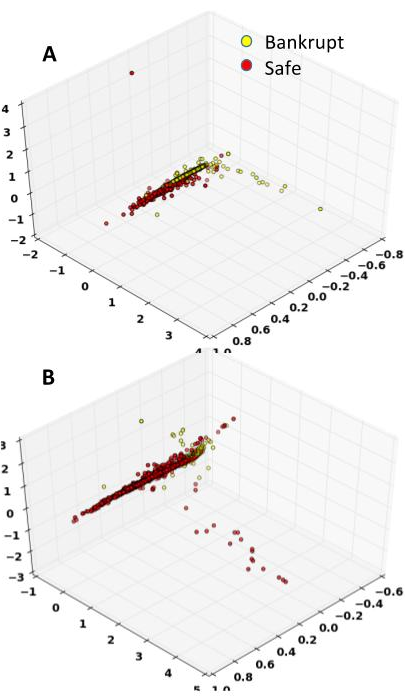
\includegraphics[width=81mm]{pca.png}
\caption{First three principal components of Original and Generated data. Figure A shows the First three principal components of the original data. Figure B shows the First three principal components of the generated data.}
\label{fig:Data}
\end{figure}


Most classification algorithms will only perform optimally when the number of samples of each class is roughly the same. Highly skewed datasets, where the minority is heavily outnumbered by one or more classes, have proven to be a challenge while at the same time becoming increasingly common. One way of addressing this issue is by re-sampling the dataset as to offset this imbalance with the hope of arriving at a more robust and fair decision boundary than one would otherwise. 


The Polish companies dataset is highly skewed. The majority (safe) class is over $97\%$ in all the 5 dataset. To overcome the skew class problem we used Synthetic Minority Over-sampling Technique (SMOTE). We implement this using imbalanced-learn package of scikit-learn contrib \cite{JMLR:v18:16-365}. 

For sampling using SMOTE, we first split our original data in $80\%-20\%$ split. We use the $80\%$ for data generation and keep the $20\%$ for the validation of our network model. Figure~\ref{fig:Data}-A. shows the first three principal components of the original data and Figure~\ref{fig:Data}-B. shows the first three principal components of the generated data. 

To model the network, we try two different approach and then compare the results obtained from the two techniques. The first technique used for learning to predict if the company is safe or bankrupt was based on the Net2Net initialization technique \cite{net2net}, which performs learning in a sequential manner starting with small MLPs and then scaling the neural network up to a larger size in width and depth by using the previous smaller network as a teacher to the new larger student network. This approach avoids the usage of a very large initial network and then re-learning the entire network from scratch if the performance is not suitable. The scaling of the network is performed by initializing the student network with the weights of the teacher network and then widening or deepening it. Widening involves adding additional neurons to a layer. Deepening involves adding a new hidden layer to the network. The advantage of the method is that it ensures that the student network improves upon the teacher network. The second approach is to train a FCN using the conventional method using the best architecture we obtain for the Net2Net approach. We will then compare the results of the two approach based on the performance metric discussed in section \ref{sec:metric}.


%we propose to treat this problem as an anomaly detection problem instead of binary classification problem. Anomaly detection (also known as outlier detection) is the identification of items, events or observations which do not conform to an expected pattern or other items in a dataset. Typically the anomalous items will translate to some kind of problem such as bank fraud, a structural defect, medical problems or errors in a text or in this case bankruptcy. Anomalies are also referred to as outliers, novelties, noise, deviations and exceptions \cite{anomaly}. In machine learning based anomaly detection we train an algorithm and obtain a model which captures the non-anomalous behaviour in the data. While testing we check if the test data can be fitted with the trained model. All the inconsistencies in fitting while testing are flagged as anomalies \cite{sakurada2014anomaly}.

%We consider safe companies as negative class (class 0) and bankrupt companies as positive class (class 1). 

%In this paper, we implement anomaly detection applying dimensionality reduction using Auto Encoders.


%Describe the computational approach -- based obviously on neural networks -- that you took to tackle the problem.


%Describe the computational experiments you conducted to validate the approach you took.
%Describe the NW Architecture
%What activations and why
%how was it optimized
%conducted on all 5 years

\begin{table*}[htb]
  \begin{center}
    \caption{Comparison of AUC score obtained using each technique}  
    \begin{tabular}{| >{\centering\arraybackslash}m{1.6in} || *5{>{\centering\arraybackslash}m{0.4in}|} @{}m{0pt}@{}}
    \hline
    \textbf{Year} & 1 & 2 & 3 & 4 & 5 &\\[2ex] 
    \hline
    \hline
    \textbf{Net2Net} & 0.967 & 0.944 &0.927 & 0.930 & 0.959 &\\[0ex]
    \hline
    \textbf{FCN} & 0.959 & 0.899 &0.903 & 0.899 & 0.945 &\\[0ex]
    \hline
    \textbf{FCN\footnote[1]{123}} & 0.543 & 0.514 &0.548 & 0.596 & 0.699 &\\[0ex]
    \hline
    \textbf{Ensemble Boosted Trees\footnote[1]{123}} & 0.959 & 0.944 &0.940 & 0.941 & 0.955 &\\[0ex]
    \hline
  \end{tabular}
  \label{tab:compare}
  \end{center}
\end{table*}
%\footnote{Footnote fdvva}
\footnotetext[1]{\cite{zikeba2016ensemble}}



\section{Metric of Performance}
\label{sec:metric}
As we discussed in section \ref{sec:proposed_method} all of the five dataset are skewed with almost $97\%$ of the majority class and rest being the other. So, in such a case, making Accuracy (that is checking $\%$ correct) as the Metric of Performance is not the right approach. The reason behind this is that the algorithm can end up predicting always the majority class and still achieve accuracy as \texttildelow$97\%$. Due to this problem we decide to use Area under the ROC curves (AUC\_ROC score) as the Metric of Performance. 

%\textbf{F1 Score:} In statistical analysis of binary classification, the F1 score (also F-score or F-measure) is a measure of a test's accuracy. It considers both the precision p and the recall r of the test to compute the score: p is the number of correct positive results divided by the number of all positive results, and r is the number of correct positive results divided by the number of positive results that should have been returned. The F1 score can be interpreted as a weighted average of the precision and recall, where an F1 score reaches its best value at 1 and worst at 0 \cite{F1}.

%\begin{align}
%  \begin{aligned}   
%  F1 = 2  \bigg( \frac{1}{\frac{1}{recall} + \frac{1}{precision}} \bigg)
%    \\
%    F1 = 2  \bigg( \frac{precision.recall}{precision + recall} \bigg)
%    \end{aligned}
% \end{align}

\textbf{Area Under the ROC Curve (AUC\_ROC):} A Receiver Operating Characteristic (ROC) curve is the most commonly used way to visualize the performance of a binary classifier \cite{dataSchool}. In statistics, a receiver operating characteristic curve, or ROC curve, is a graphical plot that illustrates the performance of a binary classifier system as its discrimination threshold is varied. The curve is created by plotting the true positive rate (TPR) against the false positive rate (FPR) at various threshold settings \cite{ROC}. Figure~\ref{fig:ROC} shows the ROC curve for year1 data of the dataset. The area under the ROC curve equals the probability that a randomly chosen positive example ranks above (is deemed to have a higher probability of being positive than) a randomly chosen negative example.

\begin{figure}[!htb]
\centering
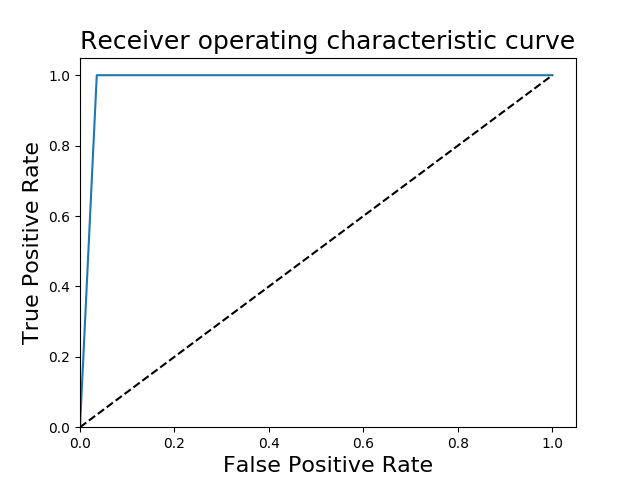
\includegraphics[width=80mm]{ROC.png}
\caption{Receiver Operating Characteristic Curve for year 1 data with the AUC score of 0.9670}
\label{fig:ROC}
\end{figure}

\section{Experiment}

\subsection{Wellness Analysis of SMOTE Data}
To confirm if the classes in the generated dataset (by SMOTE) are distributed similar to the original dataset, we implement a basic anomaly detection algorithm using Auto-Encoder with Neural Networks. For this test, we normalize all the features of the safe class and the bankrupt class separately. Then, we train the Auto-Encoder using $80\%$ safe company data of the original dataset. Then for the remaining original dataset ($20\%$ of the safe class and all of the bankrupt class) we check the reconstruction error of the dataset. Based on this error we distinguish it as safe or bankrupt. The algorithm can classify with AUC score of 0.995. Next we pass all of the generated data (SMOTE data) through the Auto-Encoder (trained on original data) and classify based on the reconstruction error. The algorithm classifies the generated data with an AUC score of 0.998. So, we confirm that both the original and generated dataset have similar distribution. We do not use this algorithm as our one of our results because we normalize the safe company data and bankrupt company data separately, thus having a prior knowledge of the data classification, to train the Auto-Encoder algorithm. 

\subsection{Model Training}

We first implement a Network model using the Net2Net technique. The technique used for training all the Net2Net networks utilized the following hyper parameters. All the models were trained with Adam as the optimizer and binary\_crossentropy was used as the cost metric to train the network. PReLu were used as the activation units as better results were obtained with this over ReLu, sigmoid and tanh. The learning rate was scheduled with initial value being the default $5\mathrm{e}{-3}$ (for Adam optimizer) and a reduction in learning rate by a factor of 10 was effected whenever the loss failed to reduce in 3 consecutive epochs. Training was performed for 2000 Epochs for each teacher network. Scaling of the network was done by widening the network first and then deepening it. Widening operation was done to a maximum of 128 neurons and then deepening operations were performed up to 8 hidden layers (discussed in detail in section \ref{sec:results}). We implemented our network models using the software package Keras \cite{chollet2015keras}. For year1 data, we start to train the network with 1 neuron and scale it to 8 hidden layers with 128 neurons in each layer. For the subsequent years, we use some of the knowledge gained in training network for year1. While training for year2, 3, 4 and 5 we chop off the network at layer4 and add layers 5, 6, 7 and 8. The intuition behind choosing to chop off at layer 4 is discussed in Section~\ref{sec:discuss}

After developing an optimized model using the Net2Net technique, we train the same network architecture using conventional method. We compare the results of the two techniques in section \ref{sec:results}. 


\section{Results}
\label{sec:results}
%Describe the results of the experiments, including their immediate implications (e.g., ``the result suggests that technique A performs better than technique B''). If your work is purely theoretical, then this section (as well as the previous section) might be replaced with mathematical proofs.

The AUC scores obtained during training is shown in Table~\ref{tab:TrainWider} (for widening operation) and Table~\ref{tab:TrainDepth} (for deepening operation). Data from Table~\ref{tab:TrainWider} indicate that the AUC score does not have a significant improvement from 64~neurons to 128~neurons during the widening operation. This is the primary reason why the widening operations were not pursued after 128~neurons. As hidden layers are added, the improvement in AUC score reduces as we add layer8. This is why we stop at layer8. All the AUC scores are reported on the $20\%$ of the original dataset which was not shown to SMOTE while sampling.

Table \ref{tab:compare} compares the results obtained by Net2Net technique with the conventional training method. It can be observed that the network trained using Net2Net technique performs better than the conventional method in all the datasets. The Table also shows the results obtained by \cite{zikeba2016ensemble} on the same dataset using FCN and Ensemble Boosted trees. Their best results for this dataset were obtained by using Ensemble Boosted Trees. We outperform their FCN for all the years and their Ensemble boosted trees for years 1 and 5.



\section{Discussion}
\label{sec:discuss}
%Describe limitations of your work as well as further-ranging implications (e.g., ``our work suggests that doing XYZ in general may be a useful approach to...'').

High AUC score for year 2,3,4 and 5 for the Net2Net in Table \ref{tab:compare} signifies that the data has some correlation over different years, thus utilizing the information learnt about the two classes during year1 helps in learning for subsequent years. 

We conducted experiments by chopping the year1 network at layer 7,6,5 and 4. We obtained best results for the years 2, 3, 4 and 5 when we chop at layer4. An intuition for this could be that the features learnt in layer5 and onwards of network 1 were highly specific to year1 which did not contribute much to the other years. But the features learnt till layer 4 were generic to all the years.



\section{Conclusions and Future Work}
%Briefly summarize the key findings your paper and point out interesting directions for future inquiry.

In this paper we show that the neural networks can be used for predictions related to the financial state of the companies with high AUC score. We also show that knowledge of one of the year's could be used to learn a model for other years. To best of our knowledge, the model presented in this paper is among the best performing kernel on this dataset. 

For future works we propose to approach this problem as an anomaly detection problem where the companies with safe functioning are non-anomalous. This approach will be able to deal with the skew class issue. Also, we feel that this problem might be able to red-flag any other financial issue and not just future bankruptcy.



%\section*{References}
%\bibliographystyle{unsrt}
\bibliographystyle{cs525}

\bibliography{9.paper}
%%%%%%%%%%%%%%%%%%%%%%%%%%%%%%%%%%%%%%%%%%%%%%%%%%%%%%%%%%%%%%%%%%%%%%%%%%%%%%%%






%\bibliography{example_paper}

\end{document} 


% This document was modified from the file originally made available by
% Pat Langley and Andrea Danyluk for ICML-2K. This version was
% created by Lise Getoor and Tobias Scheffer, it was slightly modified  
% from the 2010 version by Thorsten Joachims & Johannes Fuernkranz, 
% slightly modified from the 2009 version by Kiri Wagstaff and 
% Sam Roweis's 2008 version, which is slightly modified from 
% Prasad Tadepalli's 2007 version which is a lightly 
% changed version of the previous year's version by Andrew Moore, 
% which was in turn edited from those of Kristian Kersting and 
% Codrina Lauth. Alex Smola contributed to the algorithmic style files.  
